\subparagraph{Data Example 5: }
Finally, this last data dependency example shows the
penalty incurred due to the finite forwarding span
in an implementation.  We will assume a forwarding span
of 32 for this example.  Consider the following
code excerpt.  Note carefully the distance that each instruction
is from each other.  This distance will interact with
the finite forwarding span to create extra bubbles in
the execution of instructions even though there may be no other
constraint preventing execution from occurring earlier.

\begin{verbatim}

000	r2 <- r1 op r0
040	r3 <- r2 op r0
080	r4 <- r2 op r0
120	r5 <- r3 op r0

\end{verbatim}

The execution sequencing of this example is shown in
Figure~\ref{ex5}.

\begin{figure}
\centering
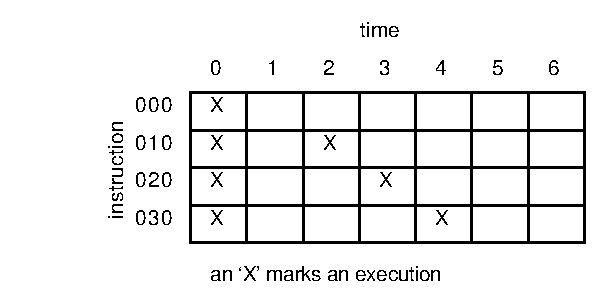
\epsfig{file=e5.eps,height=1.50in}
\caption{{\em Timing of the code example, scenario 5.}
In this example an output data broadcast is shown being
delayed by the processing of being forwarding
to a following forwarding span through the use
of the forwarding register.
Execution of an instruction at a given time is
again indicated by an `X'.}
\label{ex5}
\end{figure}

All instructions are loaded and we assume that all
instructions execute immediately and complete in one clock cycle.
Further, we assume that any of these instructions are free
from execution resource constraints to execute in any clock cycle.
The output generated from instruction 000 to register
{\tt r2}
will be broadcast on a forwarding bus and its value will be snooped
by instructions 040 and 080.  Since there is no instruction
between instruction 000 and instruction 040 that uses 
register
{\tt r2} as an input,
that output forwarding broadcast operation will result
in the output broadcast being registered in the forwarding register
located at the end of its initial forwarding span.  This
is logically after the end of active station 31 or before
the start of active station
32
(they are numbered starting at 0) in sharing group 3 (assumming
eith main-line active stations per sharing group).
The output of the forwarding register will then be broadcast
on the next forwarding span but has incurred a clock cycle delay.
This delay prevents instruction 040 from re-executing immediately
in cycle 1, due to the forwarding broadcast, and instead can only execute again in clock cycle 2
at the earliest.  The output broadcast from instruction 000
will again be registered in the forwarding register located
at the end of the second forwarding span (logically after the
end of active station 63 in sharing group 7).  
This further causes instruction 080,
which was also snooping for updates to register
{\tt r2},
to become enabled to re-execute.  We assume that it does so
at the earliest possible time which would be in clock cycle 3.
Finally, instruction 120 was snooping for updates to register
{\tt r3}.
An update to that register occurred in clock cycle 2 but because
instruction 120 is more than a forwarding span away from instruction
080, a forwarding register delay is again incurred before the update
is seen by instruction 120.  Finally, instruction 120 can execute
again, with the output from instruction 040,
at the earliest in clock cycle 4.

